\textbf{5-1} 矩形导线线圈的垂直边长为 $l$，水平边长为 $3b$，共有 $N$ 匝，构成闭合回路。今使它在磁感应强度为 $B_0$ 的水平匀强磁场中绕垂直轴旋转，角速度为 $\omega$，转轴到线圈一条垂直边的距离为 $b$，如电图5-1-1所示。

1. 试证明，在一个小的时间间隔内，线圈在转动中克服磁场作用力所作的功等于线圈中通过感应电动势消耗的能量。

2. 若线圈的电阻为 $R$，自感为 $L$，试写出线圈中的电流 $i$ 在 $t$ 时刻满足的方程，设在 $t = 0$ 时刻线圈平面与磁感线平行。当 $\omega$ 为常量时，试采用代入法验证方程有以下形式的一个解

$$
i = I_{0}\cos(\omega t + \varphi)
$$

其中 $I_0$ 和 $\varphi$ 均为常量。试证明，振幅 $I_0$ 与 $\sqrt{R^2 + \omega^2 L^2}$ 成反比，并求出初相位 $\varphi$。

3. 试分别计算线圈每转一周，电阻和电感消耗的能量。

\begin{center}
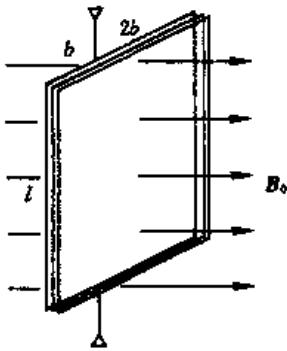
\includegraphics[width=0.2\textwidth]{figures/电图5-1-1.jpg}
\end{center}
\vfill
\newpage

\textbf{5-2} 简化的电子张弛振荡器如电图5-2-1所示。电图5-2-1中S为恒流源，输出恒定的直流电流 $I_{0}$。K是一个电子开关，它的开关动作由一个正弦讯号发生器产生的电压
$$
u_{F}(t) = U_{1} + U_{0}\sin\omega t
$$
控制，其中 $U_{1}, U_{0}$ 和 $\omega$ 都是正的常量，且 $U_{1} > U_{0}$，$u_{F}$ 只是控制 K 的开关动作，对电容 C 的充电和放电不起作用。当 $t$ 时刻 K 两端的电压亦即电容两端的电压 $u_{C}(t)$ 恰好达到 $t$ 时刻的 $u_{F}(t)$ 值时，K 自动合上，使电容器放电；当 $u_C(t)$ 直线下降，降到 $U_{\mathrm{min}}$ 时，K才自动断开。这里的 $U_{\mathrm{min}}$ 是小于 $(U_{1} - U_{0})$ 的正的常量。

1. 试在 $u \sim t$ 坐标上画出 $u_{F}(t)$ 曲线和 $U_{\min}$ 直线。设 $t = 0$ 时刻，$u_{C}(t)$ 具有任意某个不小于 $U_{\min}$ 但小于 $u_{F}(t)$ 的初始值，试在同一个 $u \sim t$ 坐标上画出 $u_{C}(t)$ 曲线。

2. 若在一定的 $I_0, U_1, U_0, \omega, U_{\min}$ 等参数值时，$u_C(t)$ 每相邻两次达到 $u_F(t)$ 的时间间隔都相等，试求每次 $u_C(t) = u_F(t)$ 时的 $u_C(t)$ 值。

\begin{center}
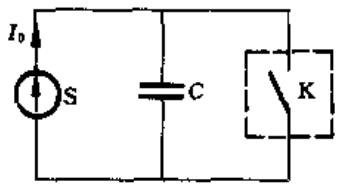
\includegraphics[width=0.2\textwidth]{figures/电图5-2-1.jpg}
\end{center}
\vfill


\textbf{5-3} 如电图5-3-1所示的电路是由下述元器件组成的：电容为 $C$ 的电容器（开始时未充电），电感为 $L$ 的线圈，电动势为 $\mathcal{E}$、内阻可略的直流电源，氖灯N，以及电键K。氖灯在其接点电压小于燃点电压 $U_{z}$ 时保持绝缘体的特性，超过 $U_{z}$ 时即点燃，并引起电容器迅速放电。当氖灯的接点电压降至熄灭点电压 $U_{g}$ 时，氖灯又成为绝缘体，并使电容放电停止。假定电容通过氖灯放电的时间非常短，以至可认为放电过程中流经线圈的电流没有变化。

设 $\mathcal{E} = 34\,\mathrm{V}$，$U_{z} = 64\,\mathrm{V}$，$U_{g} = 22\,\mathrm{V}$。试证明合上电键 K 后，氖灯 N 只亮一次。
\begin{center}
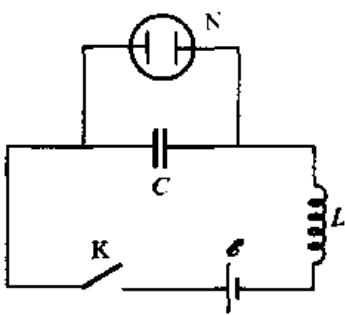
\includegraphics[width=0.2\textwidth]{figures/2bbd7c7cd10fbbb2fc0160adbaff252e22ccb2c369f2567c134a7685f8dad2ca.jpg}
\end{center}


\vfill
\newpage

\textbf{5-4} 在如电图5-4-1的电路中，适当选择电阻 $R_{1}, R_{2}, R_{3}, R_{4}$ 和电感 $L_{1}, L_{2}$，使得无论电源的电动势 $\mathcal{E}$ 是否随时间 $t$ 变化，都没有电流通过电流计 $\mathbf{M}$，设上述条件得到满足，并已知 $R_{2} = 90\,\Omega, R_{3} = 300\,\Omega, R_{4} = 60\,\Omega, L_{2} = 900\,\mathrm{mH}$。

试求 $R_{1}$ 和 $L_{1}$。
\begin{center}
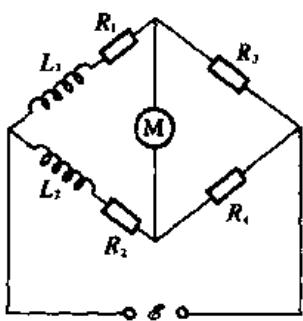
\includegraphics[width=0.18\textwidth]{figures/25ad5f3efd1ba23cc06534fc8c4b9d2871dd93a186a35a47dc8f006ea8994076.jpg}
\end{center}


\vfill


\textbf{5-5} 黑盒子内装着由电阻、电容、电感各一个组成的网络，两端点置盒外。以 $100\,\mathrm{V}$ 的直流电压接到两端，测得电流为 $0.1\,\mathrm{A}$。以 $60\,\mathrm{Hz}$、$100\,\mathrm{V}$（有效值）的交流电压接到两端，测得电流为 $1\,\mathrm{A}$（有效值）。当交流电的频率增大到 $1000\,\mathrm{Hz}$ 时，电流达到很大的极大值。试问盒内三元件是如何联接的，并求各元件的数值。
\vfill
\newpage

\textbf{5-6} 三相交流电的相电压为 $220\,\mathrm{V}$，负载是不对称的纯电阻，$R_{A}=R_{B}=22\,\Omega, R_{C}=27.5\,\Omega$，按星形联接。

1. 试求中线电流。2. 试求各线电压。3. 若中线断开，试求各线电流。
\vfill


\textbf{5-7} 一个含有非直流电源的电路如电图5-7-1所示。已知电源的电动势为 $\varepsilon(t) = 4\varepsilon_0\cos^3\omega t$，其中 $\mathcal{E}_0$ 为常量。又 $\omega$ 刚好使得 $\omega L = R$，试求 $t = 0$ 时电感 $L$ 中的电流。

\begin{center}
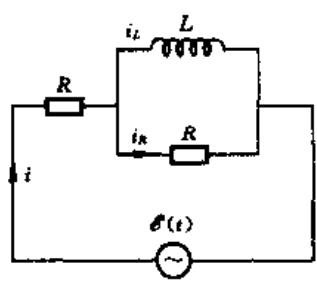
\includegraphics[width=0.3\textwidth]{figures/电图5-7-1.jpg}
\end{center}
\vfill
\newpage

\textbf{5-8} 由三个 $R$，两个 $L$，两个 $C$ 构成的交流网络，如电图5-8-1所示。当 $A$ 和 $B$ 两端加上 $U = U_0\cos(\omega t + \varphi_u)$ 的电压时，使 $\omega L = \frac{1}{\omega C} = R$。若已知 $U_{0}$ 与 $R$，试用复数法求出 $A$ 和 $B$ 之间的总阻抗（即复阻抗的模量）及流过中间（即图中 $X,Y$ 两点之间）电阻的电流的有效值。

\begin{center}
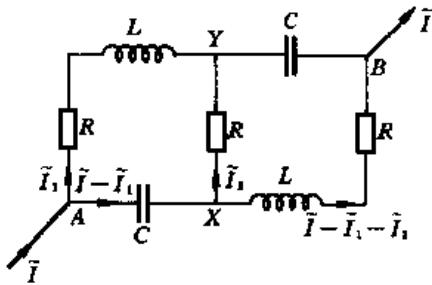
\includegraphics[width=0.3\textwidth]{figures/c2c7c82f9b3f25f03a4afda4ea17b3226fde32e830cb5d030d68a0465b436b8d.jpg}
\end{center}
\vfill


\textbf{5-9} 实际的电感元件（例如线圈）均有电阻，在通有交流电时总会有热能损耗。若将损耗的有功功率记为 $P_{\text{有功}}$，纯电感性的无功功率记为 $P_{\text{无功}}$，则元件的品质因数 $Q$ 定义为
$$
Q = \frac{P_{\text{无功}}}{P_{\text{有功}}}
$$
试求实际电感线圈的 $Q$ 值，并讨论其频率特性。
\vfill
\newpage

\textbf{5-10} 试解释"跳环"实验。

如电图5-10-1所示，竖直铁棒外绕有线圈，线圈接交流电源。铁棒上套一铝环，接通开关时，铝环会跳起来；适当调整电压，铝环会悬浮在空中。这就是"跳环"实验，试予解释。

提示：铝环有电阻和电感，应看作 RL 串联。注意分析有关简谐量的相位关系。证明铝环所受的平均作用力是斥力。

\begin{center}
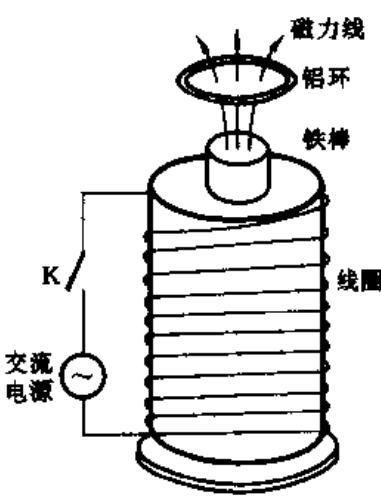
\includegraphics[width=0.2\textwidth]{figures/电图5-10-1.jpg}
\end{center}
\vfill\newpage



\textbf{5-11} 在如电图5-11-1所示的电路中，$L_{1} = 10\,\mathrm{mH}, L_{2} = 20\,\mathrm{mH}, C_{1} = 10\,\mu\mathrm{F}, C_{2} = 5\,\mu\mathrm{F}, R = 100\,\mathrm{k}\Omega$。
\begin{center}
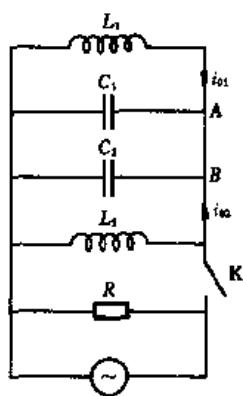
\includegraphics[width=0.15\textwidth]{figures/bb627b8a51c5a98501e3c8cf761b49523d8888aaf009a7aa86ee4ba1c7af9127.jpg}
\end{center}
开关 K 长时间闭合。电源的正弦式频率 $f$ 可改变但其电流振幅保持不变。

1. 以 $f_{\mathrm{m}}$ 表示有功功率为极大值 $P_{\max}$ 时的频率，以 $f_{+}$ 和 $f_{-}$ 分别表示有功功率为 $\frac{1}{2}P_{\max}$ 时的两个频率。试确定 $f_{m}$ 和 $\Delta f = f_{+} - f_{-}$ 的比值。

打开开关 K，在开关打开 $t$ 时间后，通过 $L_{1}$ 和 $L_{2}$ 的电流分别为 $i_{01}=0.1\,\mathrm{A}$，$i_{02}=0.2\,\mathrm{A}$，电压 $U_{0}=40\,\mathrm{V}$。

2. 试计算电路 $L_{1}C_{1}C_{2}L_{2}$ 的固有振荡频率。

3. 试确定导线 $AB$ 内的电流.

4. 试计算线圈 $L_{1}$ 中的电流振荡的振幅。

\vfill\newpage

\textbf{5-12} 角频率为 $\omega$ 的正弦交流电电流波沿着如电图5-12-1所示的无限 $LC$ 网络传播，相邻两电容上的交流电压的相移均为 $\varphi$ .

1. 试确定 $\varphi$ 对 $\omega, L, C$ 的函数关系。

2. 如果每个网络的长度为 $l$ ，试求电流波的传播速度。

3. 试说明在什么条件下电流波的传播速度几乎与 $\omega$ 无关，并求出这种情况下电流波的传播速度。
\begin{center}
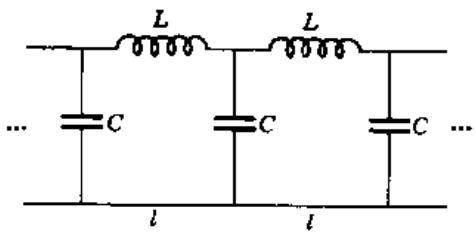
\includegraphics[width=0.25\textwidth]{figures/电图5-12-1.jpg}
\end{center}
\vfill


\textbf{5-13} 如电图5-13-1所示是一对互感耦合的 $LR$ 电路。试证明，在无漏磁条件下，两电路充、放电的时间常量都是
$$
\tau = \frac{L_{1}}{R_{1}} + \frac{L_{2}}{R_{2}}
$$
\begin{center}
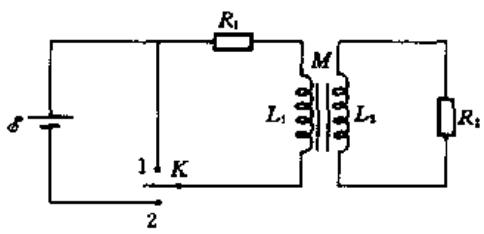
\includegraphics[width=0.25\textwidth]{figures/电图5-13-1.jpg}
\end{center}
\vfill\newpage

\textbf{5-14} 在如电图5-14-1所示的电路中，各元件的值均已标明。设在 $t = 0$ 时刻，$A$ 到 $B$ 的电压值为 $U_{10}$，$B$ 到 $D$ 的电压值为 $U_{20}$。试求尔后 $A$ 和 $B$ 之间的电压随时间 $t$ 的变化。

\begin{center}
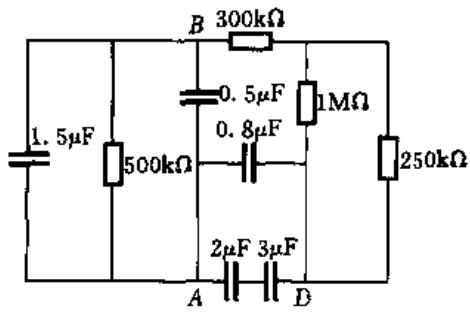
\includegraphics[width=0.2\textwidth]{figures/电图5-14-1.jpg}
\end{center}
\vfill


\textbf{5-15} 在如电图5-15-1所示的电路中，A和B为放大器的输入端，P为输出端，输出电压 $U_{P}$ 取决于A和B之间的电势差 $(U_{A}-U_{B})$，其间的关系如电图5-15-2所示。

1. 设开始时电键 K 断开，放大器尚未工作，电容 C 中也不带电荷，且可变电阻器阻值 $R_{2}=0$，然后将 K 迅速合上并立即断开，使放大器被触发而开始工作。试求放大器输出的电流 $I_{P}$ 随时间 $t$ 的变化。

\begin{center}
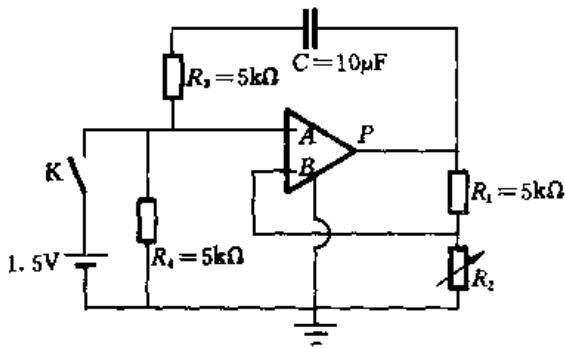
\includegraphics[width=0.3\textwidth]{figures/电图5-15-1.jpg}
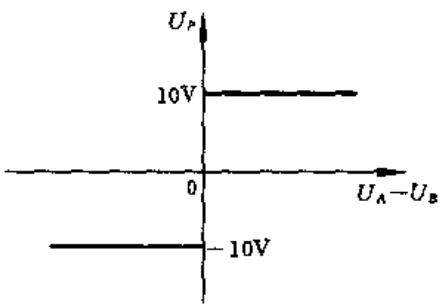
\includegraphics[width=0.3\textwidth]{figures/电图5-15-2.jpg}
\end{center}
\vfill\newpage

\textbf{5-16} 两个理想电容器 $C_1$ 和 $C_2$ 串联起来接在直流电源上，电压分配为 $U_1:U_2 = C_2:C_1$。实际电容器都有一定的漏阻，漏阻相当于并联在理想电容器 $C_1, C_2$ 上的电阻 $R_1, R_2$。当漏阻趋于无穷时，实际电容器趋于理想电容器。将两个实际电容器接在直流电源上，根据稳恒条件，电压分配应为 $U_1:U_2 = R_1:R_2$。设 $C_1:C_2 = R_1:R_2 = 1:2$，并设想 $R_1$ 和 $R_2$ 按此比例趋于无穷。试问，这时电压分配 $U_1:U_2$ 如何？一种看法认为，这时两个电容器都是理想的，故应为 $U_1:U_2 = C_2:C_1 = 2:1$。另一种看法认为，电压的分配只与 $R_1$ 和 $R_2$ 的比值有关，而此比值不变，故当 $R_1 \to \infty$ 及 $R_2 \to \infty$ 时，电压分配仍应为 $U_1:U_2 = R_1:R_2 = 1:2$。试问，哪一种看法正确。
\vfill


\textbf{5-17} 电路如电图5-17-1所示，开始时断路，电容器上无电量，在 $t = 0$ 时刻合上电键K。已知交流电源的电动势为
$$
\mathcal{E} = \mathcal{E}_{0}\cos(\omega t + \varphi_{\mathcal{E}})
$$
试求电流随时间 $t$ 的变化 $i(t)$。
\begin{center}
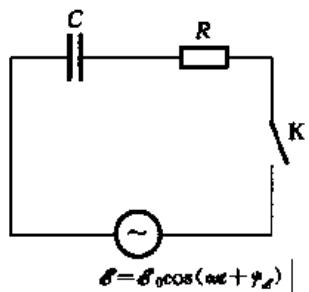
\includegraphics[width=0.2\textwidth]{figures/45175b3d0913ef07c003e429591ac5ccb5ddf76a7b8ec45198fcf5912d84b41e.jpg}
\end{center}


\vfill\newpage

\textbf{5-18} 按照静电学的观点，可以认为地球表面是良导体。设地球表面所带总电量为 $Q_{0}$，平均面电荷密度为 $\sigma_0$。

1. 天气晴好时，大气中有一垂直向下的电场，记为 $E$，在地球表面附近其值约为 $E_{0} = 150\,\mathrm{V/m}$。试求地球表面的面电荷密度 $\sigma_{0}$ 和地球表面所带的总电量 $Q_{0}$。

2. 电场强度的绝对值随着高度的增加而减小，在距地面 $100\,\mathrm{m}$ 的高度处，场强约为 $100\,\mathrm{V/m}$。试求 $100\,\mathrm{m}$ 高度处与地球表面之间每立方米大气中的平均净电荷量。

3. 在第2问中求出的净电荷体密度，实际上是数值几乎相等的单位体积内单价正离子（数密度为 $n_{+}$）的电量和负离子（数密度为 $n_{-}$）的电量的代数和。天气晴好时，在地面附近 $n_{+}\approx n_{-}=6\times 10^{8}\,\mathrm{m^{-3}}$。这些离子会在竖直向下电场的作用下运动，它们（实指其中的正离子）的运动速度 $v$ 与场强 $E$ 的关系为
$$
v \approx 1.5\times 10^{-4}E
$$

式中 $v$ 的单位取 $\mathrm{m/s}$，$E$ 的单位取 $\mathrm{V/m}$。若无其他过程（例如闪电）为地球表面充电，试问因大气中离子的运动需经多长时间才能使地球表面的电荷中和掉一半。

4. 用如电图5-18-1所示的实验装置，可以测出大气中的电场强度 $E$ 和地球表面的面电荷密度 $\sigma$。

\begin{center}
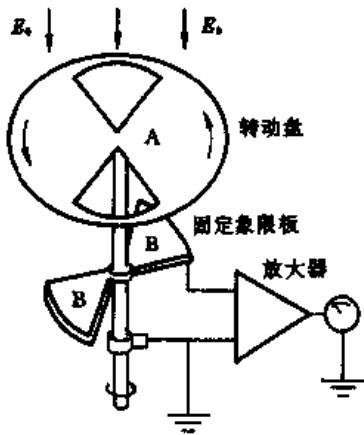
\includegraphics[width=0.2\textwidth]{figures/电图5-18-1.jpg}
\end{center}
\vfill

